\newcommand{\TeamNo}{31}

\newcommand{\HWno}{04}

\newcommand{\AuthorOneName}{Merve Nur Öztürk}
\newcommand{\AuthorOneID}{2311322}

\newcommand{\AuthorTwoName}{Atakan Süslü}
\newcommand{\AuthorTwoID}{2311371}

\newcommand{\AuthorThreeName}{Betül Rana Kuran}
\newcommand{\AuthorThreeID}{2311173}


\documentclass[letterpaper,12pt]{article}
\usepackage{tabularx} % extra features for tabular environment
\usepackage{amsmath}  % improve math presentation
\usepackage{amssymb}
\usepackage{xcolor}
\usepackage{float}
\usepackage[export]{adjustbox}
\usepackage{graphicx} % takes care of graphic including machinery
\usepackage[margin=1in,letterpaper]{geometry} % decreases margins
\usepackage{cite} % takes care of citations

\begin{document}
\begin{center}
AE 305, 2020-21 Fall \hfill \textbf{HW \HWno} \hfill \textbf{Team \TeamNo} \\
\noindent\rule{\textwidth}{0.4pt}
\begin{tabular}{p{0.33\textwidth} | p{0.33\textwidth} | p{0.33\textwidth} }
	\AuthorOneName&\AuthorTwoName&\AuthorThreeName\\
	\textit{\AuthorOneID}&\textit{\AuthorTwoID}&\textit{\AuthorThreeID}
\end{tabular}
\noindent\rule{\textwidth}{0.4pt}
\end{center}

%Report start

\section{Introduction}
Finite Difference Method uses finite difference relations which are obtained from Taylor
series expansions in order to approximate the partial derivatives in a partial differential
equation. The equations representing the partial differentials are called Finite Difference
Equations. In this homework, given a convection diffusion wave equation:

\begin{equation}
	\frac{\partial \omega}{\partial t} + V\frac{\partial \omega}{\partial x} = \nu\frac{\partial^2 \omega}{\partial x^2}
	\label{eqn:gaussian}
\end{equation}

where V is the constant convection velocity, and $\nu$ is the diffusion (viscosity) coefficient,
and $\omega$ is distributed initially as follows:
\begin{equation}
	\omega(x,t=0) = exp(-b ln2(x/\Delta x)^2)
\end{equation}

where $\Delta x = 0.1$, and $b = 0.025$, it is requested to solve Equation \ref{eqn:gaussian} by modifying the given fortran code and
using forward-time central-space FDE, and prove that the equation is conditionally stable by
using different $\sigma$ (Courant number) and d values where $\sigma$ and d values are as the following:

\begin{eqnarray}
	\sigma &=& \frac{V\Delta t}{\Delta x} \nonumber \\
	d &=& \frac{\nu\Delta t}{\Delta x^2}
\end{eqnarray}
It is also asked to solve both Equation \ref{eqn:gaussian} and convection equation, where d equals
zero, by forward-time backward-space FDE and compare the solution. Afterwards, given a high order
accuracy FDE, first it is requested to perform consistency analysis on it and then solving
Equation \ref{eqn:gaussian} by using this FDE:

\begin{eqnarray}
\frac{-\omega^{n+1}_{i}+4\omega^{n}_{i}-3\omega^{n-1}_{i}}{2\Delta t} + V\frac{\omega^{n}_{i+1}-\omega^{n}_{i-1}}{2\Delta x} = \nu\frac{\omega^{n}_{i+1}-2\omega^{n}_{i}+\omega^{n}_{i-1}}{\Delta x^2}
\end{eqnarray}

Finally, implicit FDE (backward-time central-space) is used to solve Equation \ref{eqn:gaussian}.
In all solutions the range of x is such that -L/2$\leq$x$\leq$L/2 where L=40.


\section{Method}
\subsection{Finite Difference Method}
Finite Difference method is used to solve partial differential equations by 
approximating partial derivatives in these equations with finite difference relations.
In this homework, 1-D, linear, convection diffusion equation and convection equation are solved
with combination of finite difference approximations.
\begin{equation}
	\frac{\partial w}{\partial t} + V\frac{\partial w}{\partial x}=\nu\frac{\partial^2 w}{\partial x^2}
	\label{eqn:cde}
\end{equation}
is convective diffusion equation and
\begin{equation}
	\frac{\partial w}{\partial t} + V\frac{\partial w}{\partial x}=0 
	\label{eqn:ce}
\end{equation}
is convective equation.\\
Two different derivations is used for the explicit finite difference equation of 
Equation \ref{eqn:cde} in this homework.The first derivation of FDE is also used for the explicit 
FDE of Equation \ref{eqn:ce}. In both derivations, the first term of
the equation forward time approximation is used.
\begin{equation}
	\frac{\partial w}{\partial t}\vert^{n}=\frac{w^{n+1}-{w^n}}{\Delta t}+O(\Delta t)
	\label{eqn:ft}
\end{equation}
In the first derivation, for second and third terms of the Equation \ref{eqn:cde}, 
central space approximations of
$\frac{\partial w}{\partial x}\vert_{i}$ of order ($\Delta x^2$) and 
$\frac{\partial^2 w}{\partial x^2}\vert_{i}$ of order ($\Delta x^2$), respectively, are used.
\begin{equation}
	\frac{\partial w}{\partial x}\vert_{i}=\frac{w_{i+1}-w_{i-1}}{2\Delta x}+O(\Delta x^2)
	\label{eqn:cs1}
\end{equation}
\begin{equation}
	\frac{\partial^2 w}{\partial x^2}\vert_{i}=\frac{w_{i+1}-2w_i+w_{i-1}}{\Delta x^2}+O(\Delta x^2)
	\label{eqn:cs2}
\end{equation}
By substituting Equation \ref{eqn:ft}, \ref{eqn:cs1}, and \ref{eqn:cs2} into Equation \ref{eqn:cde}, it becomes:
\begin{equation}
	\frac{w_{i}^{n+1}-{w_{i}^{n}}}{\Delta t}+\frac{w_{i+1}^{n}-w_{i-1}^{n}}{2\Delta x}
	=\frac{w_{i+1}^{n}-2w_{i}^{n}+w_{i-1}^{n}}{\Delta x^2}+O(\Delta x^2, \Delta t)
\end{equation}
The explicit FDE of Equation \ref{eqn:cde} based on forward time and central spatial differences is obtained:
\begin{equation}
	w_{i}^{n+1}= w_{i}^{n}-\frac{\sigma}{2}(w_{i+1}^{n}-w_{i-1}^{n})+d(w_{i+1}^{n}-2w_{i}^{n}+w_{i-1}^{n})+O(\Delta x^2,\Delta t)
\end{equation}
where $\sigma = \frac{V\Delta t}{\Delta x }$ and $d = \frac{\nu\Delta t}{\Delta x^2 }$.
\\To derive the explicit FDE of Equation \ref{eqn:ce}, Equation \ref{eqn:ft} and \ref{eqn:cs1} are
substituted into Equation \ref{eqn:ce}
\begin{equation}
	\frac{w_{i}^{n+1}-{w_{i}^{n}}}{\Delta t}+\frac{w_{i+1}^{n}-w_{i-1}^{n}}{2\Delta x}
	=0+O(\Delta x^2, \Delta t)
\end{equation}
The explicit FDE of Equation \ref{eqn:ce} based on forward time and central spatial differences is obtained:
\begin{equation}
	w_{i}^{n+1}= w_{i}^{n}-\frac{\sigma}{2}w_{i+1}^{n}-w_{i-1}^{n}+O(\Delta x^2, \Delta t)
\end{equation}
where $\sigma = \frac{V\Delta t}{\Delta x }$.
\\In the second derivation, instead of central space approximation, backward space approximation is used.
Backward space approximation of $\frac{\partial w}{\partial x}\vert$ of order ($\Delta x$)
\begin{equation}
	\frac{\partial w}{\partial x}\vert_{i}=\frac{w_{i}-w_{i-1}}{\Delta x}+O(\Delta x)
	\label{eqn:bs1}
\end{equation}
Backward space approximation of $\frac{\partial^2 w}{\partial x^2}\vert$ of order ($\Delta x$)
\begin{equation}
	\frac{\partial^2 w}{\partial x^2}\vert_{i}=\frac{w_{i}-2w_{i-1}+w_{i-2}}{\Delta x^2}+O(\Delta x)
	\label{eqn:bs2}
\end{equation}
By substituting Equation \ref{eqn:ft}, \ref{eqn:bs1}, and \ref{eqn:bs2} into Equation \ref{eqn:cde}
\begin{equation}
	\frac{w_{i}^{n+1}-{w_{i}^{n}}}{\Delta t}+\frac{w_{i}^{n}-w_{i-1}^{n}}{\Delta x}
	=\frac{w_{i}^{n}-2w_{i-1}^{n}+w_{i-2}^{n}}{\Delta x^2}+O(\Delta x,\Delta t)
\end{equation}
The explicit FDE of Equation \ref{eqn:cde} based on forward time and backward spatial
differences is obtained:
\begin{equation}
	w_{i}^{n+1}= w_{i}^{n}-\sigma(w_{i+1}^{n}-w_{i-1}^{n})+d(w_{i}^{n}-2w_{i-1}^{n}+w_{i-2}^{n})+O(\Delta x,\Delta t)
\end{equation}
where $\sigma = \frac{V\Delta t}{\Delta x }$ and $d = \frac{\nu\Delta t}{\Delta x^2 }$.
\\ To obtain the implicit FDE of Equation \ref{eqn:cde}, backward time central space method is used.
Backward time difference is used for the first term of Equation \ref{eqn:cde}
\begin{equation}
	\frac{\partial w}{\partial t}\vert^{n}=\frac{w^{n}-w^{n-1}}{\Delta x}+O(\Delta t)
	\label{eqn:bt}
\end{equation}
Equation \ref{eqn:cs1} and \ref{eqn:cs2} are used to approximate the second and third
terms of Equation \ref{eqn:cde}, respectively. Equation \ref{eqn:bt}, \ref{eqn:cs1}
and \ref{eqn:cs2} are inserted in the Equation \ref{eqn:cde}
\begin{equation}
	\frac{w_{i}^{n}-{w_{i}^{n-1}}}{\Delta t}+\frac{w_{i+1}^{n-1}-w_{i-1}^{n-1}}{2\Delta x}
	=\frac{w_{i+1}^{n-1}-2w_{i}^{n-1}+w_{i-1}^{n-1}}{\Delta x^2}+O(\Delta x^2, \Delta t)
\end{equation}
To define a PDE as implicit, it should be discretized at time level $n+1$. So, equation becomes
\begin{equation}
	\frac{w_{i}^{n+1}-{w_{i}^{n}}}{\Delta t}+\frac{w_{i+1}^{n+1}-w_{i-1}^{n+1}}{2\Delta x}
	=\frac{w_{i+1}^{n+1}-2w_{i}^{n+1}+w_{i-1}^{n+1}}{\Delta x^2}+O(\Delta x^2, \Delta t)	
\end{equation}
The implicit FDE of Equation \ref{eqn:cde} based on BTCS Euler Implicit method is obtained:
\begin{equation}
	-(\frac{\sigma}{2}+d)w_{i-1}^{n+1}+(2d+1)w_{i}^{n+1}+(\frac{\sigma}{2}-d)w_{i+1}^{n+1} = w_{i}^{n}
\end{equation}
where $\sigma = \frac{V\Delta t}{\Delta x }$ and $d = \frac{\nu\Delta t}{\Delta x^2 }$.
\newpage
\section{Results and Discussion}
\subsection{Stability of the Solution of the Explicit FDE of Convection Diffusion Equation}
\begin{figure}[!ht] 
	\centering 
	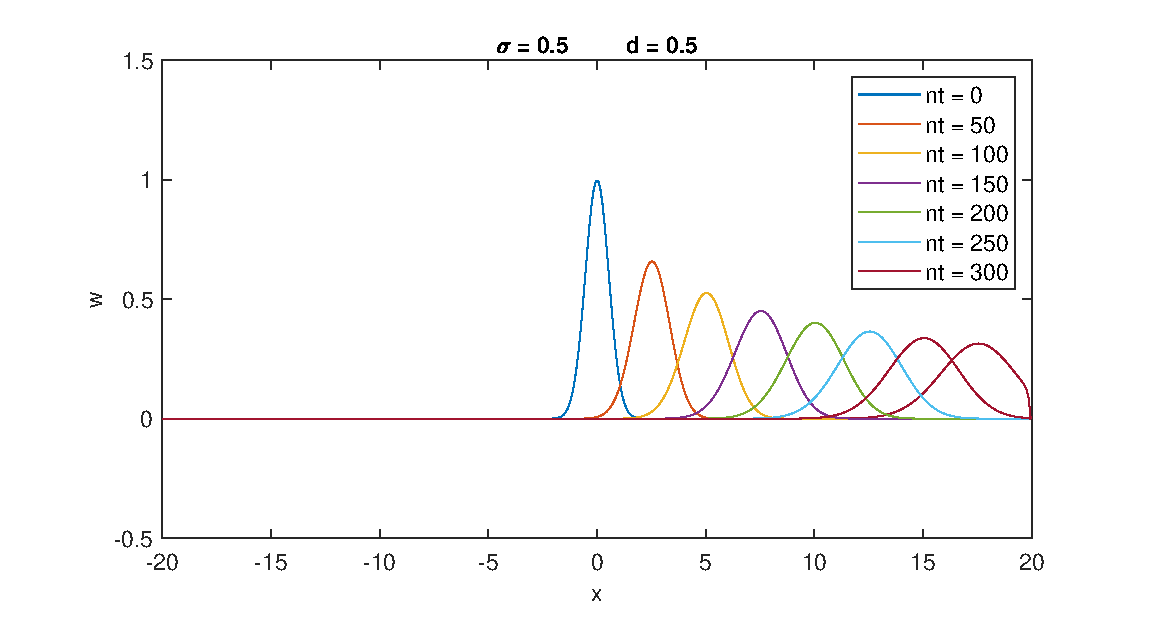
\includegraphics[max height=8.5cm]{graphs/FTCS/ConvectionDiffusion/sigma05d05.eps}
	\caption{Convection diffusion solution by the explicit FTCS method with $\sigma= 0.5$ and $d=0.5$ at different time steps.}
 	\label{fig:FTCSsigma05d05}
\end{figure}
\begin{figure}[!ht] 
	\centering 
	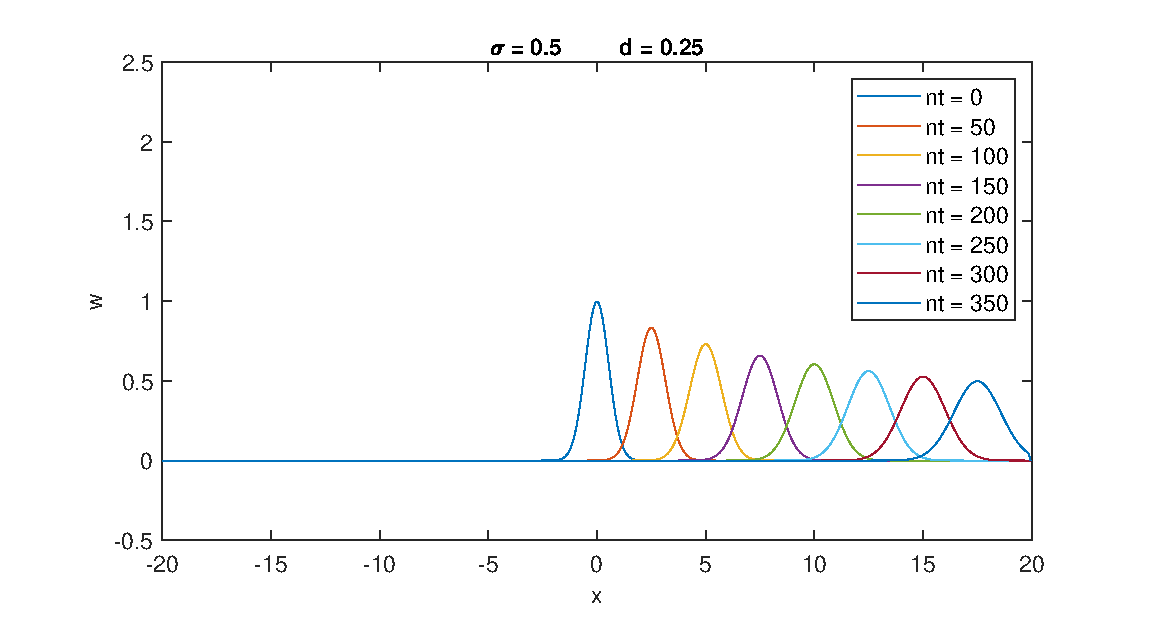
\includegraphics[max height=8.5cm]{graphs/FTCS/ConvectionDiffusion/sigma05d025.eps}
	\caption{Convection diffusion solution by the explicit FTCS method with $\sigma= 0.5$ and $d=0.25$ at different time steps.}
	 \label{fig:FTCSsigma05d025}
\end{figure}
\newpage
\begin{figure}[!ht] 
	\centering 
	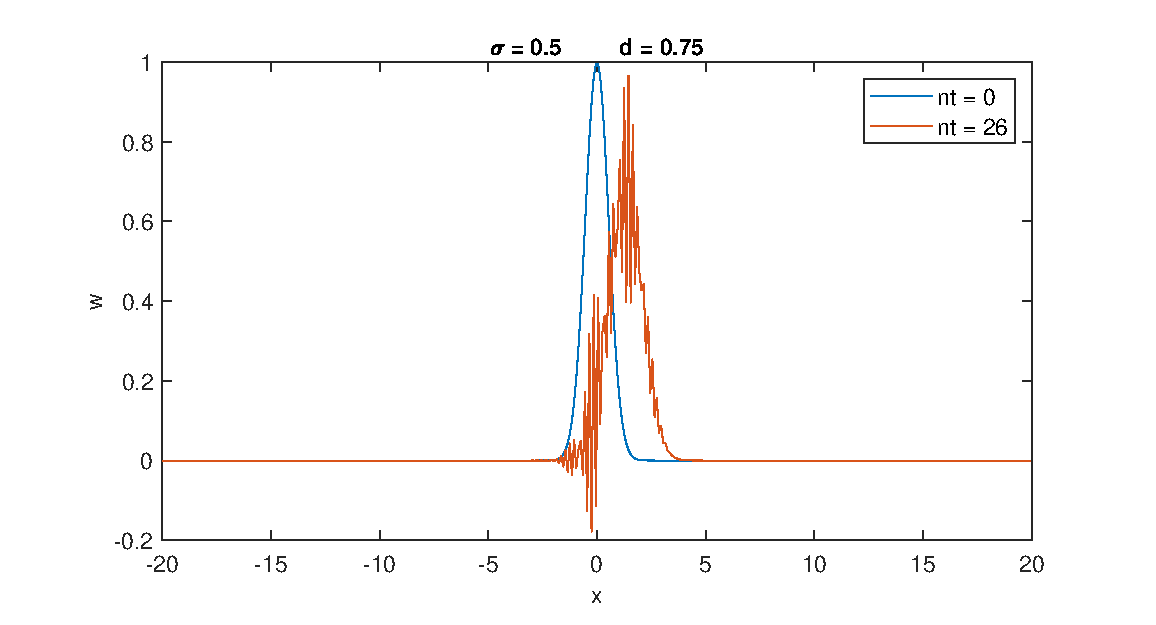
\includegraphics[max height=8.5cm]{graphs/FTCS/ConvectionDiffusion/sigma05d075.eps}
	\caption{Convection diffusion solution by the explicit FTCS method with $\sigma= 0.5$ and $d=0.75$ at $nt=0$ and $nt=25$.}
	 \label{fig:FTCSsigma05d075}
\end{figure}
\begin{figure}[!ht] 
	\centering 
	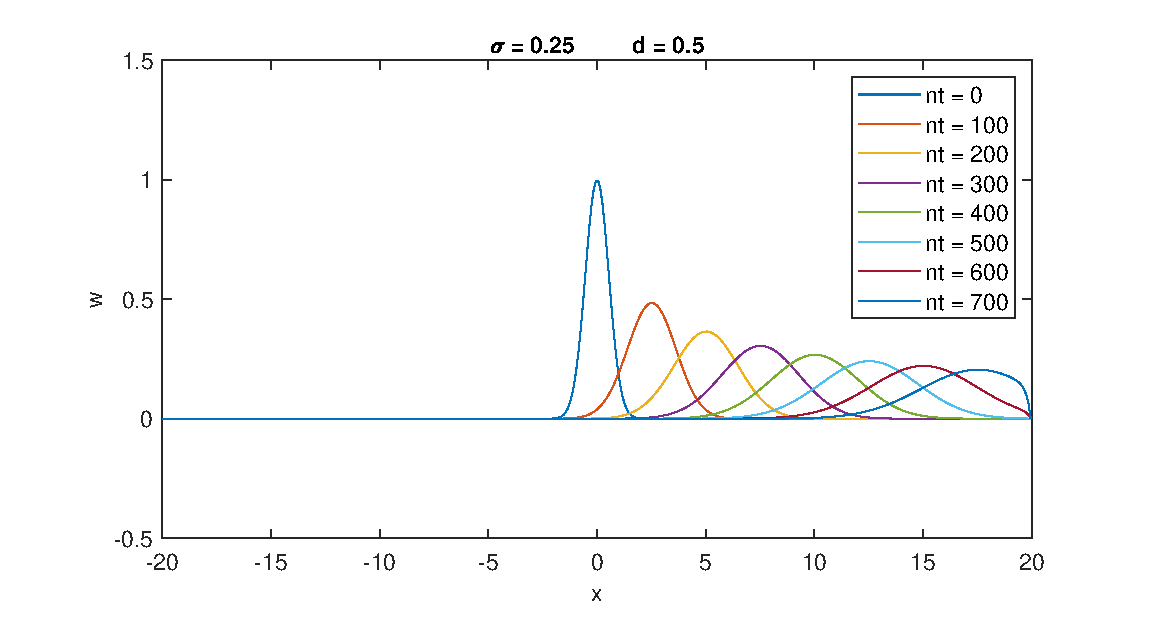
\includegraphics[max height=8.5cm]{graphs/FTCS/ConvectionDiffusion/sigma025d05.eps}
	\caption{Convection diffusion solution by the explicit FTCS method with $\sigma= 0.25$ and $d=0.5$ at different time steps.}
	 \label{fig:FTCSsigma025d05}
\end{figure}
\newpage
\begin{figure}[!ht] 
	\centering 
	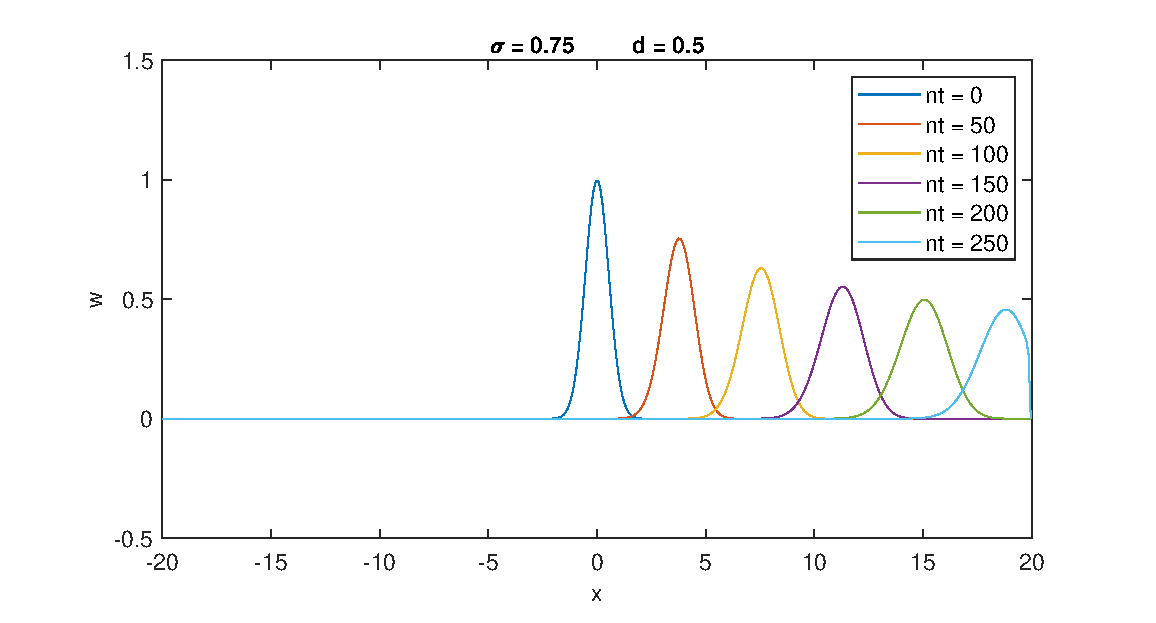
\includegraphics[max height=8.5cm]{graphs/FTCS/ConvectionDiffusion/sigma075d05.eps}
	\caption{Convection diffusion solution by the explicit FTCS method with $\sigma= 0.75$ and $d=0.5$ at different time steps.}
	 \label{fig:FTCSsigma075d05}
\end{figure}
\begin{figure}[!ht] 
	\centering 
	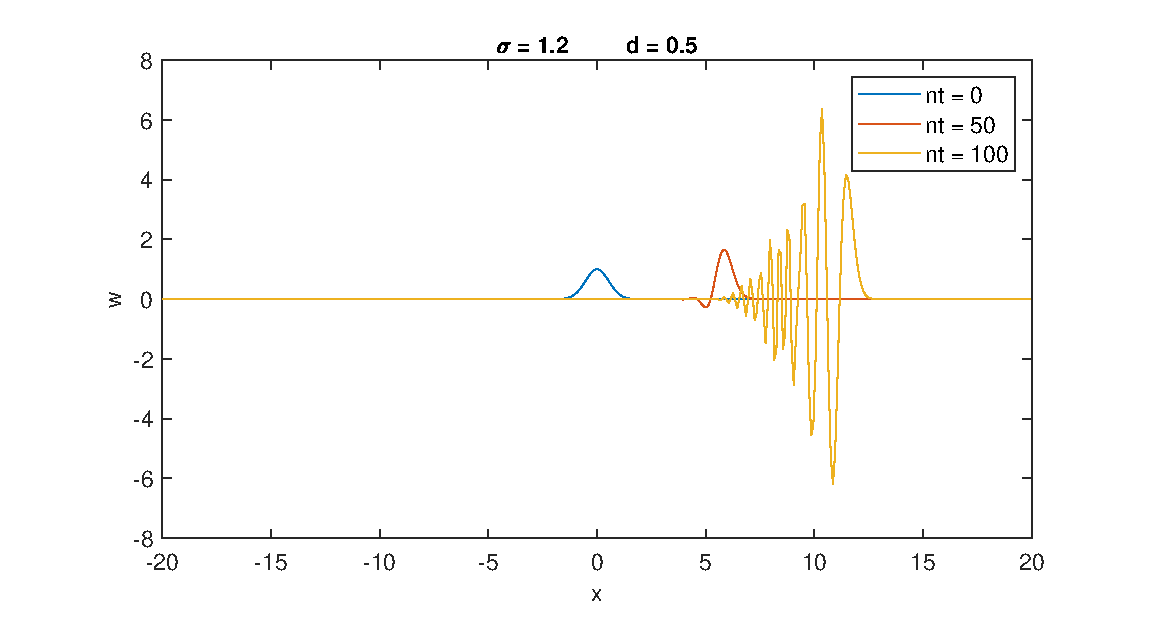
\includegraphics[max height=8.5cm]{graphs/FTCS/ConvectionDiffusion/sigma12d05.eps}
	\caption{Convection diffusion solution by the explicit FTCS method with $\sigma= 1.2$ and $d=0.5$ at different time steps.}
	 \label{fig:FTCSsigma12d05}
\end{figure}
\newpage

Figure \ref{fig:FTCSsigma05d05} shows the solution of the explicit FTCS
method for Equation \ref{eqn:cde} with $\sigma= 0.5$ and $d=0.5$ at various time steps.
Figure \ref{fig:FTCSsigma05d025} shows the solution of the same explicit FDE but with 
different d value ($d=0.25$) at various time steps. As can be seen from the Figure \ref{fig:FTCSsigma05d05}
and \ref{fig:FTCSsigma05d025}, as time step increases, both curves continue to oscillate with a decrease in their
amplitudes. It can be seen that the solution of the expilicit FDE is convergent for $d=0.5$
and $d=0.25$ while keeping $\sigma$ constant and equal to 0.5. Since the stability is a condition
to be satisfied for convergence, it can be understood that both solutions are stable. \\
\indent Figure \ref{fig:FTCSsigma05d075} shows the solution of the explicit FTCS
method for Equation \ref{eqn:cde} with $\sigma= 0.5$ and $d=0.75$ at the initial condition
and $25^{th}$ time step. The curve in the graph has some deterioration at $nt = 25$. Therefore,
the explicit FDE is unstable for $\sigma= 0.5$ and $d=0.75$.\\
\indent Figure \ref{fig:FTCSsigma025d05} and Figure \ref{fig:FTCSsigma075d05} illustrates the solutions of the explicit FTCS
method for Equation \ref{eqn:cde} for $d=0.5$ with different sigma values, $\sigma= 0.25$ and $\sigma=0.75$,
respectively, at various time steps. In both Figure \ref{fig:FTCSsigma025d05}
and \ref{fig:FTCSsigma075d05}, the wave lengths of curves increases and the amplitudes of the waves are reduced
with increasing time steps. Overall, it can be said that the solution of the explicit is convergent, hence stable 
FDE for $d=0.5$ and $\sigma = 0.25$, and $\sigma = 0.25$ since there is no distortion observed.\\
\indent Figure \ref{fig:FTCSsigma12d05} demonstrates the solution of the explicit FTCS
method for Equation \ref{eqn:cde} with $\sigma= 1.2$ and $d=0.5$ at various time steps. For the curve in the
Figure \ref{fig:FTCSsigma12d05}, the amplitude of the wave increases and the wave becomes distrupted with 
increasing time step. Consequently, the solution of the explicit FDE is unstable for $\sigma=1.2$ and $d=0.5$\\
\indent To conclude this subsection, since the explicit FDE of the convection diffusion equation is stable for some $d$ 
and $\sigma$ values whereas it can be unstable for some other combinations of $d$ and $\sigma$ values, it is conditionally stable.
\newpage
\subsection{Comparison of convective eqution with FTBS}
Figures \ref{fig:FTBSsigma025d0}, \ref{fig:FTBSsigma05d0}, \ref{fig:FTBSsigma075d0}, and \ref{fig:FTBSsigma12d0}
demonstrate solutions of convection equation using FTBS with different $\sigma$ values at various time
steps. It can be observed that for $\sigma$ values less than 1.2, the solutions obtained are convergent.
However, for $\sigma = 1.2$, wave curve is distorted and the solution is divergent. Besides, comparing Figures
\ref{fig:FTBSsigma025d0}, \ref{fig:FTBSsigma05d0}, and \ref{fig:FTBSsigma075d0}, it can be seen that the
amplitudes of the wave curves decrease faster, whereas the wave lengths of the curves experience a more rapid
increase for smaller $\sigma$ values.
\begin{figure}[!ht] 
	\centering 
	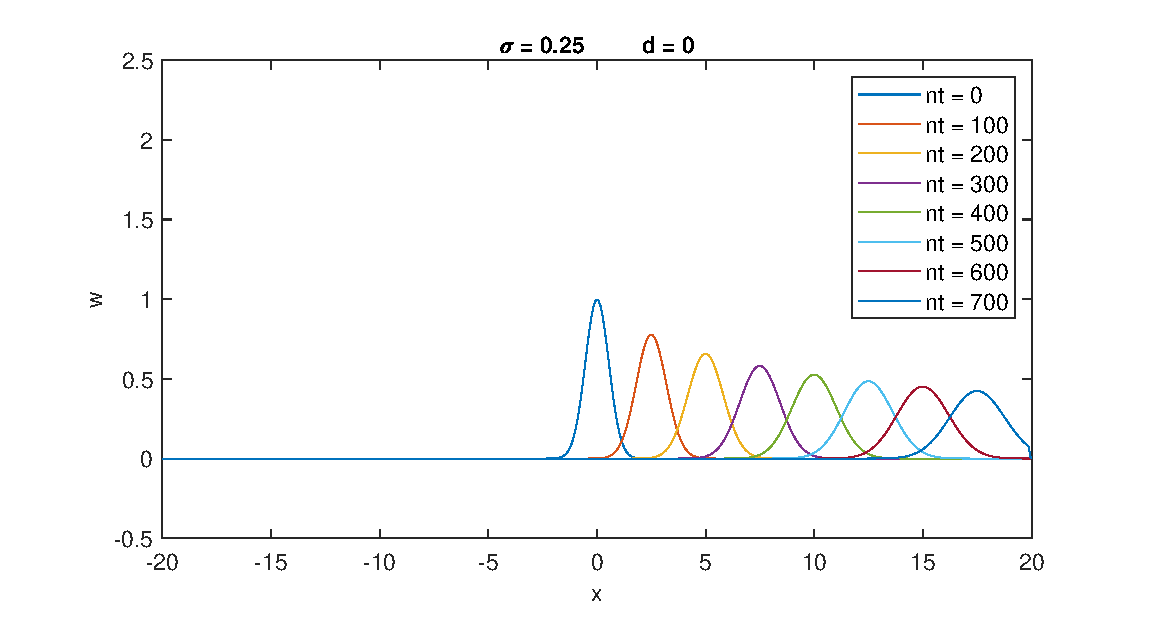
\includegraphics[max height=8.5cm]{graphs/FTBS/Convection/sigma025d0.eps}
	\caption{Convection solution by the explicit FTBS method with $\sigma= 0.25$ at different time steps.}
	 \label{fig:FTBSsigma025d0}
\end{figure}
\begin{figure}[!ht] 
	\centering 
	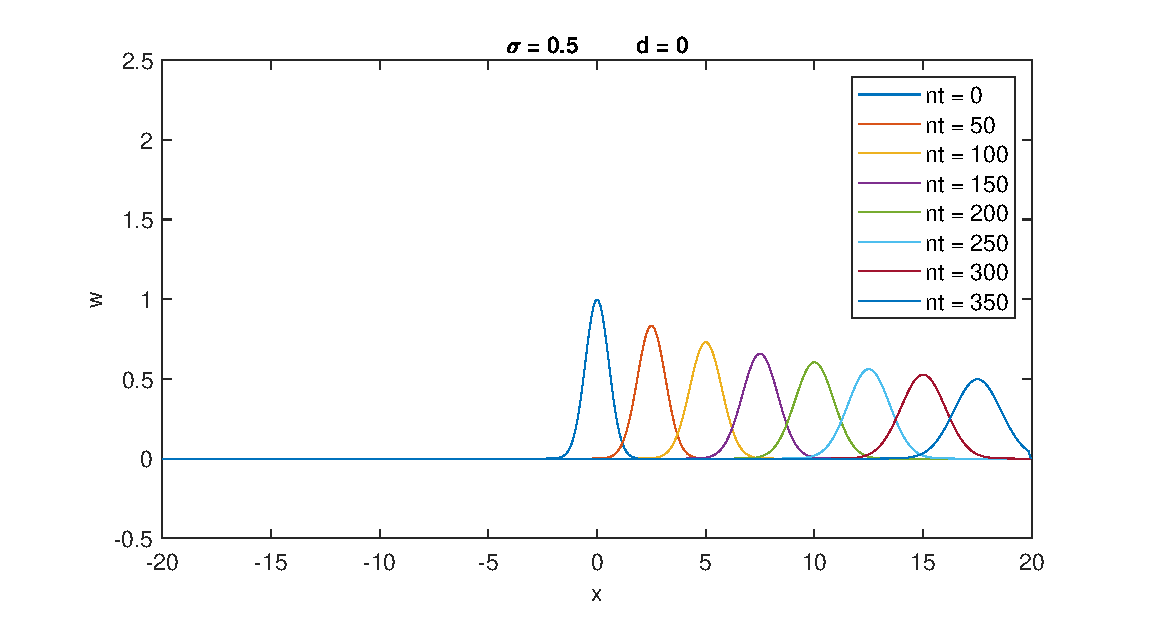
\includegraphics[max height=8.5cm]{graphs/FTBS/Convection/sigma05d0.eps}
	\caption{Convection solution by the explicit FTBS method with $\sigma= 0.5$ at different time steps.}
	 \label{fig:FTBSsigma05d0}
\end{figure}
\newpage
\begin{figure}[!ht] 
	\centering 
	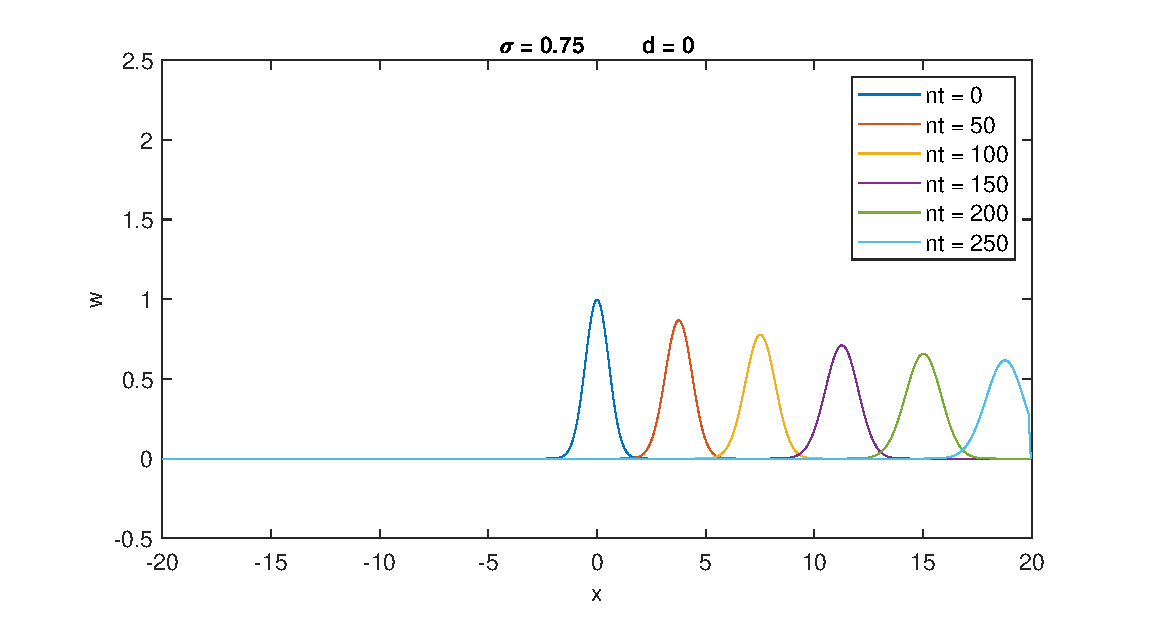
\includegraphics[max height=8.5cm]{graphs/FTBS/Convection/sigma075d0.eps}
	\caption{Convection solution by the explicit FTBS method with $\sigma= 0.75$ at different time steps.}
	 \label{fig:FTBSsigma075d0}
\end{figure}
\begin{figure}[!ht] 
	\centering 
	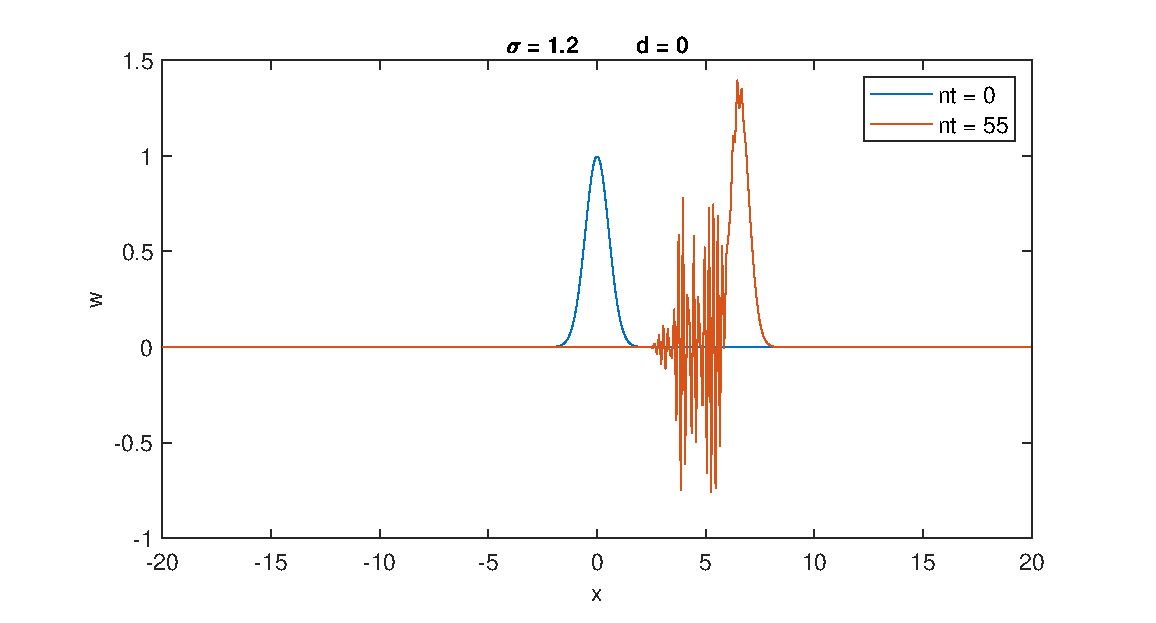
\includegraphics[max height=8.5cm]{graphs/FTBS/Convection/sigma12d0.eps}
	\caption{Convection diffusion solution by the explicit FTBS method with $\sigma= 1.2$ at $nt=0$ and $nt=55$.}
	 \label{fig:FTBSsigma12d0}
\end{figure}
\newpage
Figures \ref{fig:FTBSsigma025d05}, \ref{fig:FTBSsigma05d05}, \ref{fig:FTBSsigma075d05}, and \ref{fig:FTBSsigma12d05}
illustrate the solutions of convection diffusion equation using FTBS with various $\sigma$ values at different time
steps while keeping d value constant. As can be seen from these figures, for $\sigma = 1.2$, a convergent solution
is obtained for the convection diffusion equation. Nonetheless, for $\sigma$ values smaller than 1.2, calculations
gave divergent solutions. 
\\
\indent Figures \ref{fig:FTBSsigma12d05}, \ref{fig:FTBSsigma12d025}, and \ref{fig:FTBSsigma12d075} monitor the 
solutions of convection diffusion equation using FTBS with various d values at different time steps
while keeping $\sigma$ value constant. When the d value is decreased to 0.25 from 0.5, the solution remains
convergent. Nevertheless, if the d value is increased, such as 0.75, distortion in wave curve is observed and
the solution obtained is divergent. Comparing Figures \ref{fig:FTBSsigma12d05} and \ref{fig:FTBSsigma12d025},
it is observed that the decrease in the amplitude of the waves is more significant for higher d values. In addition,
the wave length increases faster for d = 0.5 compared to the increase in the wave length for d = 0.25.
\begin{figure}[!ht] 
	\centering 
	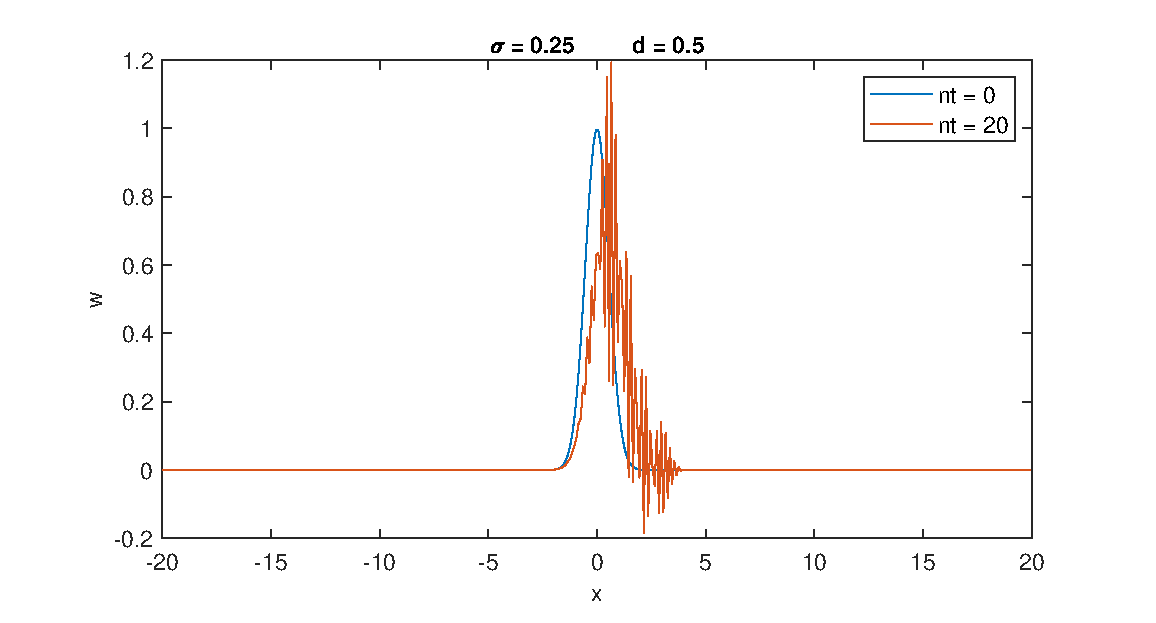
\includegraphics[max height=8.5cm]{graphs/FTBS/ConvectionDiffusion/sigma025d05.eps}
	\caption{Convection diffusion solution by the explicit FTBS method with $\sigma= 0.25$ and $d=0.5$ at different time steps.}
	 \label{fig:FTBSsigma025d05}
\end{figure}
\begin{figure}[!ht] 
	\centering 
	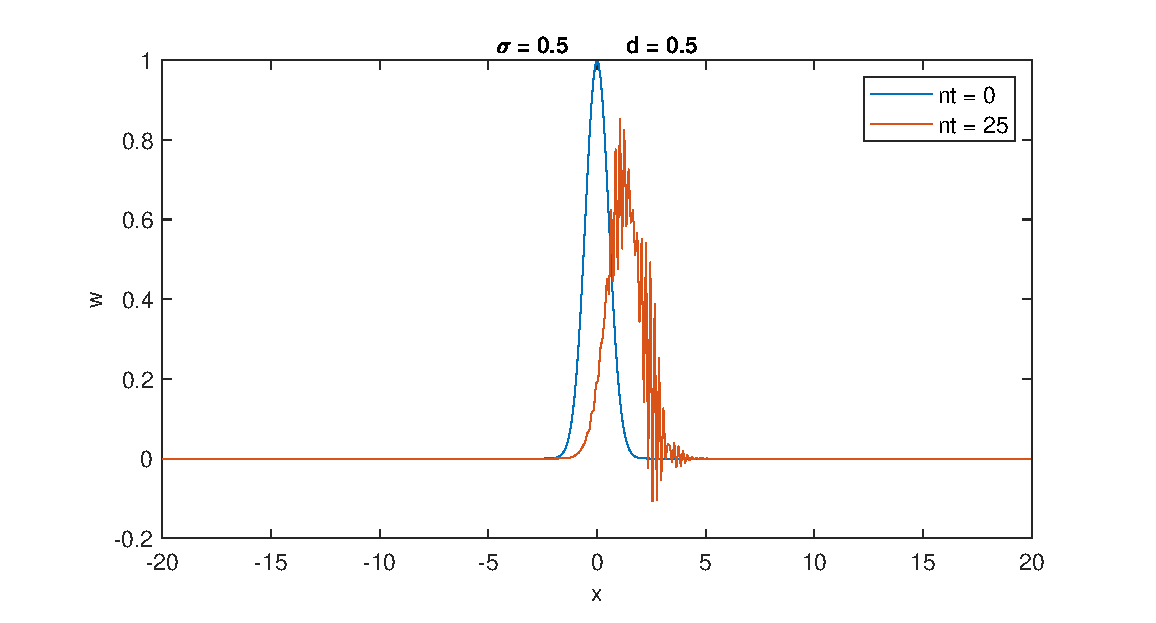
\includegraphics[max height=8.5cm]{graphs/FTBS/ConvectionDiffusion/sigma05d05.eps}
	\caption{Convection diffusion solution by the explicit FTBS method with $\sigma= 0.5$ and $d=0.5$ at different time steps.}
	 \label{fig:FTBSsigma05d05}
\end{figure}
\newpage
\begin{figure}[!ht] 
	\centering 
	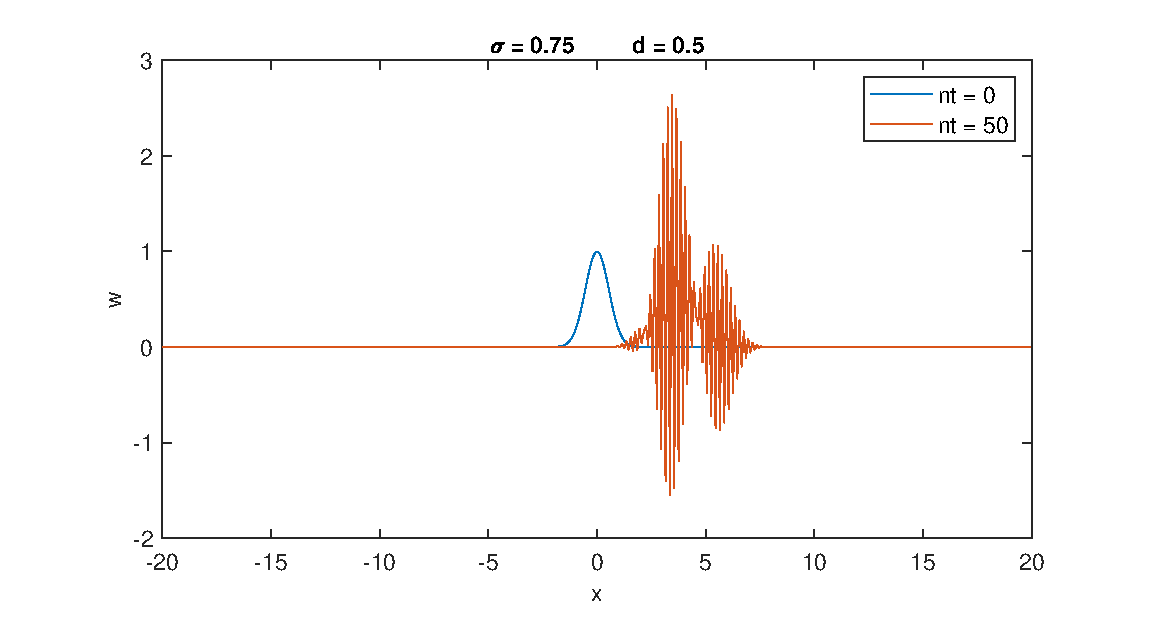
\includegraphics[max height=8.5cm]{graphs/FTBS/ConvectionDiffusion/sigma075d05.eps}
	\caption{Convection diffusion solution by the explicit FTBS method with $\sigma= 0.75$ and $d=0.5$ at different time steps.}
	 \label{fig:FTBSsigma075d05}
\end{figure}
\begin{figure}[!ht] 
	\centering 
	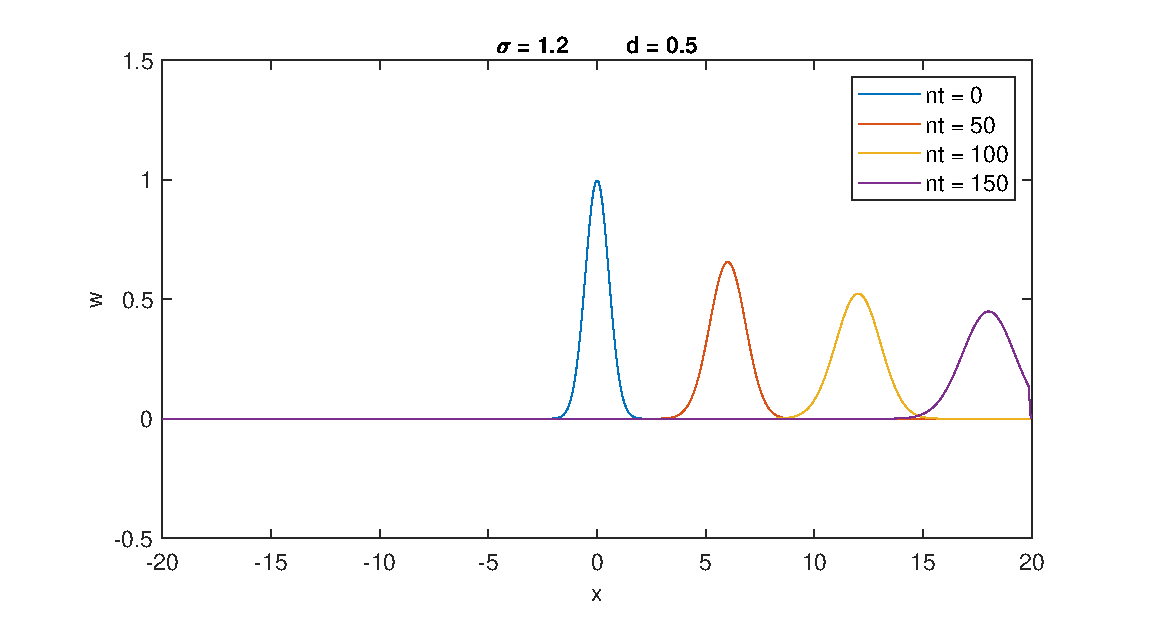
\includegraphics[max height=8.5cm]{graphs/FTBS/ConvectionDiffusion/sigma12d05.eps}
	\caption{Convection diffusion solution by the explicit FTBS method with $\sigma= 1.2$ and $d=0.5$ at different time steps.}
	 \label{fig:FTBSsigma12d05}
\end{figure}
\newpage
%\begin{figure}[!ht] 
%	\centering 
%	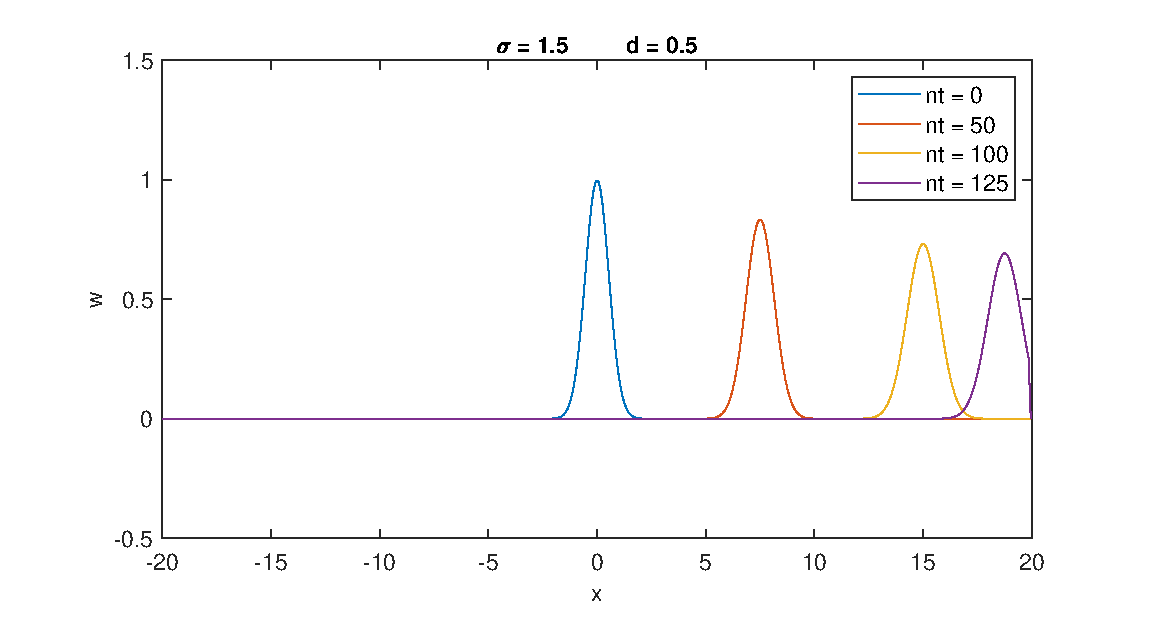
\includegraphics[max height=8.5cm]{graphs/FTBS/ConvectionDiffusion/sigma15d05.eps}
%	\caption{Convection diffusion solution by the explicit FTBS method with $\sigma= 1.5$ and $d=0.5$ at different time steps.}
%	 \label{fig:FTBSsigma15d05}
%\end{figure}
\begin{figure}[!ht] 
	\centering 
	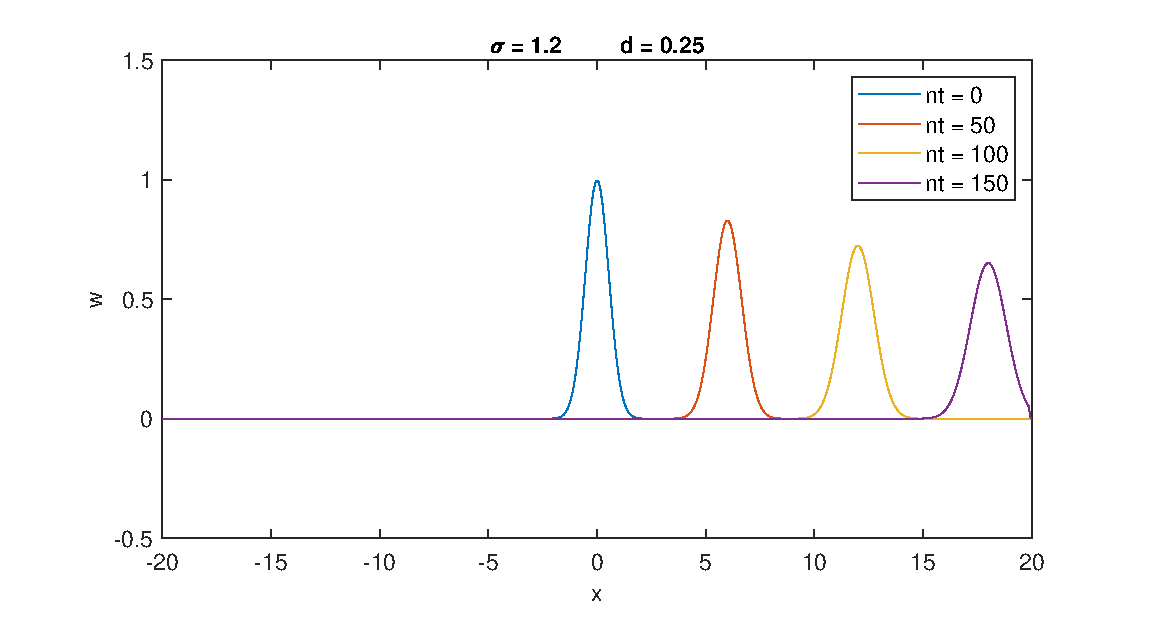
\includegraphics[max height=8.5cm]{graphs/FTBS/ConvectionDiffusion/sigma12d025.eps}
	\caption{Convection diffusion solution by the explicit FTBS method with $\sigma= 1.2$ and $d=0.25$ at different time steps.}
	 \label{fig:FTBSsigma12d025}
\end{figure}
\newpage
\begin{figure}[!ht] 
	\centering 
	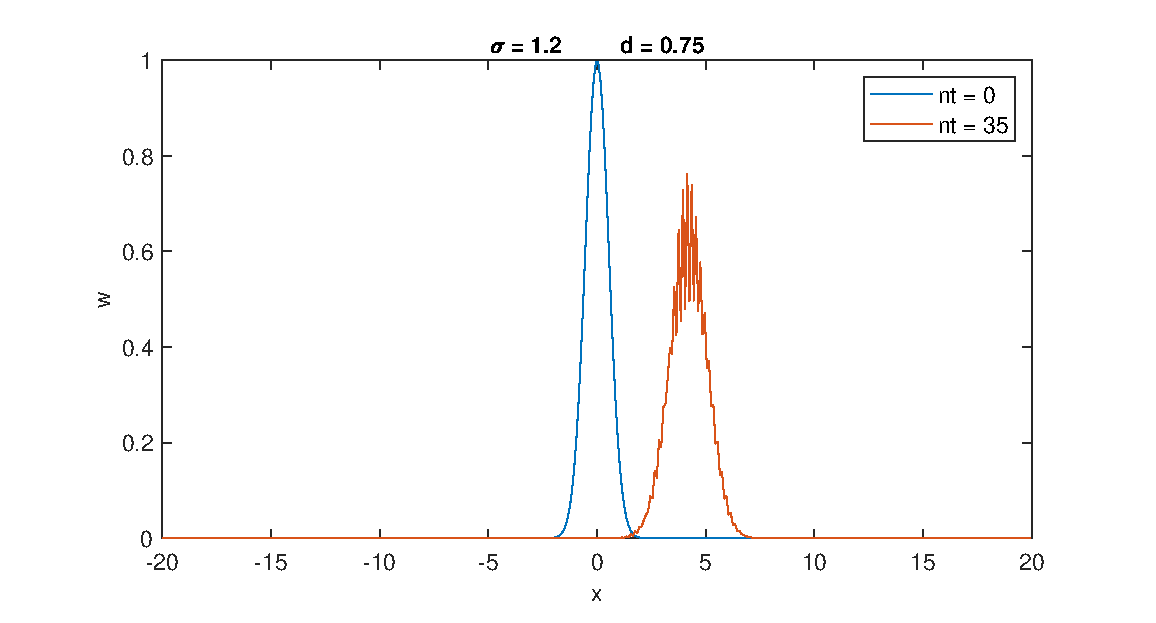
\includegraphics[max height=8.5cm]{graphs/FTBS/ConvectionDiffusion/sigma12d075.eps}
	\caption{Convection diffusion solution by the explicit FTBS method with $\sigma= 1.2$ and $d=0.75$ at different time steps.}
	 \label{fig:FTBSsigma12d075}
\end{figure}

Overall, if the solutions of the convection diffusion equation and the convection equation are
compared, it can be denoted that for $\sigma$ values lower than 1.2 the FTBS equation gives convergent
solutions for the convection equation whereas for the convection diffusion equation the solutions
obtained by FTBS equation is divergent.


\newpage
\subsection{Consistency Analysis of the Given FDE}
Consistency is one of the conditions to be able to approximate to the PDE. What is meant by consistency is
that as the step sizes goes to zero, FDE should converge to the PDE. For a given FDE written at a point
(i,n), consistency analysis is to expand the discrete values with Taylor series expansions, and leaving
the original PDE terms on the left hand-side and all the other terms on the right hand-side. If the right
hand side goes to zero as the step sizes goes to zero, the FDE is consistent. This precedure is carried
out for the following FDE: 

\begin{equation}
	\frac{-\omega^{n+1}_{i}+4\omega^{n}_{i}-3\omega^{n-1}_{i}}{2\Delta t} + V\frac{\omega^{n}_{i+1}-\omega^{n}_{i-1}}{2\Delta x} = \nu\frac{\omega^{n}_{i+1}-2\omega^{n}_{i}+\omega^{n}_{i-1}}{\Delta x^2}
	\label{equation:q4}
\end{equation}

First, all terms except the $\omega^{n}_{i}$ term, are expanded aorund $\omega^{n}_{i}$ with TSE:

\begin{eqnarray}
	\omega^{n+1}_i &=& w^n_i + \Delta t \omega_t|^n_i + \frac{\Delta t^2}{2} \omega_{tt}|^n_i + \frac{\Delta t^3}{6} \omega_{ttt}|^n_i ... \nonumber \\
	\omega^{n-1}_i &=& w^n_i - \Delta t \omega_t|^n_i + \frac{\Delta t^2}{2} \omega_{tt}|^n_i - \frac{\Delta t^3}{6} \omega_{ttt}|^n_i ... \nonumber \\
	\omega^n_{i+1} &=& w^n_i + \Delta x \omega_x|^n_i + \frac{\Delta x^2}{2} \omega_{xx}|^n_i + \frac{\Delta x^3}{6} \omega_{xxx}|^n_i ... \nonumber \\
	\omega^n_{i-1} &=& w^n_i - \Delta x \omega_x|^n_i + \frac{\Delta x^2}{2} \omega_{xx}|^n_i - \frac{\Delta x^3}{6} \omega_{xxx}|^n_i ... 
\end{eqnarray}

Then the above relations are substituted into Equation \ref{equation:q4}:

\begin{equation}
	\omega_t|^n_i - \Delta t \omega_{tt}|^n_i + \frac{\Delta t^2}{6} \omega_{ttt}|^n_i + V\omega_x|^n_i + V\frac{\Delta x^2}{6}\omega_{xxx}|^n_i = \nu\omega_{xx}|^n_i + O(\Delta t^4,\Delta x^4)
\end{equation}

Collecting the original PDE terms to the RHS:

\begin{equation}
	[\omega_t + V\omega_x - \nu\omega_{xx}]|^n_i = \Delta t \omega_{tt}|^n_i - \frac{\Delta t^2}{6} \omega_{ttt}|^n_i - V\frac{\Delta x^2}{6}\omega_{xxx}|^n_i + O(\Delta t^4,\Delta x^4)
\end{equation}

Since the right hand-side terms goes to zero as $\Delta t$ and $\Delta x$ approach to zero, the FDE given
in Equation \ref{equation:q4} is consistent.

\section{Conclusion}

\end{document}